\documentclass[letterpaper, 10pt, draftclsnofoot, onecolumn]{IEEEtran}
\usepackage[latin1]{inputenc}
\usepackage[T1]{fontenc}
\usepackage[english]{babel}
\usepackage{amsmath}
\usepackage{amssymb,amsfonts,textcomp}
\usepackage{color}
\usepackage{array}
\usepackage{comment}
\usepackage{supertabular}
\usepackage{hhline}
\usepackage{hyperref}
\def\name{Steven Powers, Josh Matteson, Evan Tschuy}
\hypersetup{colorlinks=true, linkcolor=blue, citecolor=blue, filecolor=blue, urlcolor=blue, pdfauthor = {\name},
  pdfkeywords = {cs461 ``senior capstone'' requirements},
  pdftitle = {CS 461 Requirements Document},
  pdfsubject = {CS 461 Requirements Document},
  pdfpagemode = UseNone}
\usepackage[pdftex]{graphicx}
% Outline numbering
\setcounter{secnumdepth}{5}
\renewcommand\thesection{\arabic{section}}
\renewcommand\thesubsection{\arabic{section}.\arabic{subsection}}
\renewcommand\thesubsubsection{\arabic{section}.\arabic{subsection}.\arabic{subsubsection}}
\renewcommand\theparagraph{\arabic{section}.\arabic{subsection}.\arabic{subsubsection}.\arabic{paragraph}}

\makeatletter
\newcommand\arraybslash{\let\\\@arraycr}
\makeatother
% Page layout (geometry)
\setlength\voffset{-1in}
\setlength\hoffset{-1in}
\setlength\topmargin{0.5in}
\setlength\oddsidemargin{1in}
\setlength\evensidemargin{1in}
\setlength\textheight{8.278in}
\setlength\textwidth{6.5in}
\setlength\footskip{0.561in}
\setlength\headheight{0.5in}
\setlength\headsep{0.461in}
% Footnote rule
\setlength{\skip\footins}{0.0469in}
\renewcommand\footnoterule{\vspace*{-0.0071in}\setlength\leftskip{0pt}\setlength\rightskip{0pt plus 1fil}\noindent\textcolor{black}{\rule{0.25\columnwidth}{0.0071in}}\vspace*{0.0398in}}
% Pages styles
\makeatletter
\newcommand\ps@Standard{
  \renewcommand\@oddhead{\selectlanguage{english}\rmfamily\color{black}Admix - Many Voices Publishing Platform\hfill \hfill }
  \renewcommand\@evenhead{\@oddhead}
  \renewcommand\@oddfoot{\foreignlanguage{english}{\textcolor{black}{SSRS Page }}\foreignlanguage{english}{\textcolor{black}{\thepage{}}}}
  \renewcommand\@evenfoot{\@oddfoot}
  \renewcommand\thepage{\arabic{page}}
}
\newcommand\ps@Convertviii{
  \renewcommand\@oddhead{}
  \renewcommand\@evenhead{\@oddhead}
  \renewcommand\@oddfoot{}
  \renewcommand\@evenfoot{\@oddfoot}
  \renewcommand\thepage{\arabic{page}}
}
\newcommand\ps@Convertvii{
  \renewcommand\@oddhead{}
  \renewcommand\@evenhead{\@oddhead}
  \renewcommand\@oddfoot{}
  \renewcommand\@evenfoot{\@oddfoot}
  \renewcommand\thepage{\arabic{page}}
}
\newcommand\ps@Convertvi{
  \renewcommand\@oddhead{}
  \renewcommand\@evenhead{\@oddhead}
  \renewcommand\@oddfoot{}
  \renewcommand\@evenfoot{\@oddfoot}
  \renewcommand\thepage{\arabic{page}}
}
\newcommand\ps@Convertv{
  \renewcommand\@oddhead{}
  \renewcommand\@evenhead{\@oddhead}
  \renewcommand\@oddfoot{}
  \renewcommand\@evenfoot{\@oddfoot}
  \renewcommand\thepage{\arabic{page}}
}
\newcommand\ps@Convertiv{
  \renewcommand\@oddhead{}
  \renewcommand\@evenhead{\@oddhead}
  \renewcommand\@oddfoot{}
  \renewcommand\@evenfoot{\@oddfoot}
  \renewcommand\thepage{\arabic{page}}
}
\newcommand\ps@Convertii{
  \renewcommand\@oddhead{}
  \renewcommand\@evenhead{\@oddhead}
  \renewcommand\@oddfoot{}
  \renewcommand\@evenfoot{\@oddfoot}
  \renewcommand\thepage{\arabic{page}}
}
\newcommand\ps@FirstPage{
  \renewcommand\@oddhead{}
  \renewcommand\@evenhead{\@oddhead}
  \renewcommand\@oddfoot{}
  \renewcommand\@evenfoot{\@oddfoot}
  \renewcommand\thepage{\arabic{page}}
}
\makeatother
\pagestyle{Standard}
\setlength\tabcolsep{1mm}
\renewcommand\arraystretch{1.3}
% footnotes configuration
\makeatletter
\renewcommand\thefootnote{\arabic{footnote}}
\makeatother
\title{MANY VOICES PUBLISHING PLATFORM}
\author{Steven Powers}
\date{2016-10-27}


\begin{document}
\clearpage\setcounter{page}{1}\pagestyle{Standard}
\thispagestyle{FirstPage}


\bigskip


\bigskip

\clearpage{\centering\selectlanguage{english}\bfseries\color{black}\LARGE
SYSTEMS AND SOFTWARE \ REQUIREMENTS SPECIFICATION (SSRS) FOR
\par}


\bigskip

{\centering\selectlanguage{english}\bfseries\color{black}
MANY VOICES PUBLISHING PLATFORM
\par}


\bigskip


\bigskip


\bigskip


\bigskip

{\centering\selectlanguage{english}\bfseries\color{black}
Version 0.5
\par}

{\centering\selectlanguage{english}\bfseries\color{black}
October 27, 2016
\par}


\bigskip


\bigskip

{\centering\selectlanguage{english}\bfseries\color{black}
Prepared for:
\par}

{\centering\selectlanguage{english}\bfseries\color{black}
Dr. Carlos Jensen, D. Kevin McGrath, and Dr. Kirsten Winters
\par}

{\centering\selectlanguage{english}\bfseries\color{black}
CS461 Senior Capstone
\par}


\bigskip


\bigskip

{\centering\selectlanguage{english}\bfseries\color{black}
Prepared by:
\par}

{\centering\selectlanguage{english}\bfseries\color{black}
Commix
\par}

{\centering\selectlanguage{english}\bfseries\color{black}
Josh Matteson, Steven Powers, and Evan Tschuy
\par}

{\centering\selectlanguage{english}\bfseries\color{black}
Oregon State University
\par}

{\centering\selectlanguage{english}\bfseries\color{black}
Corvallis, OR \ 97330
\par}

\begin{comment}
\clearpage{\centering\selectlanguage{english}\bfseries\color{black}
Many Voices Publishing Platform SSRS
\par}


\bigskip

{\centering\selectlanguage{english}\bfseries\color{black}
RECORD OF CHANGES
\par}


\bigskip

\begin{flushleft}
\tablehead{}
\begin{supertabular}{|m{0.47685984in}|m{0.6087598in}|m{1.3587599in}|m{0.23375985in}|m{2.0462599in}|m{0.7337598in}|m{0.6330598in}|}
\hline
~

\centering \selectlanguage{english}\color{black} Change number &
~

\centering \selectlanguage{english}\color{black} Date completed &
~

\centering \selectlanguage{english}\color{black} Location of change
(e.g., page or figure \#) &
\centering \selectlanguage{english}\bfseries\color{black} A\newline
M\newline
D &
~

~

\centering \selectlanguage{english}\color{black} Brief description of
change &
~

\centering \selectlanguage{english}\color{black} Approved by (initials)
&
~

\centering\arraybslash \selectlanguage{english}\color{black} Date
Approved\\\hline
~
 &
~
 &
~
 &
~
 &
~
 &
~
 &
~
\\\hline
~
 &
~
 &
~
 &
~
 &
~
 &
~
 &
~
\\\hline
~
 &
~
 &
~
 &
~
 &
~
 &
~
 &
~
\\\hline
~
 &
~
 &
~
 &
~
 &
~
 &
~
 &
~
\\\hline
~
 &
~
 &
~
 &
~
 &
~
 &
~
 &
~
\\\hline
~
 &
~
 &
~
 &
~
 &
~
 &
~
 &
~
\\\hline
~
 &
~
 &
~
 &
~
 &
~
 &
~
 &
~
\\\hline
~
 &
~
 &
~
 &
~
 &
~
 &
~
 &
~
\\\hline
~
 &
~
 &
~
 &
~
 &
~
 &
~
 &
~
\\\hline
~
 &
~
 &
~
 &
~
 &
~
 &
~
 &
~
\\\hline
~
 &
~
 &
~
 &
~
 &
~
 &
~
 &
~
\\\hline
\end{supertabular}
\end{flushleft}
{\selectlanguage{english}\color{black}
\foreignlanguage{english}{*}\foreignlanguage{english}{\textbf{A}}\foreignlanguage{english}{
- ADDED
\ }\foreignlanguage{english}{\textbf{M}}\foreignlanguage{english}{ -
MODIFIED
\ }\foreignlanguage{english}{\textbf{D}}\foreignlanguage{english}{ -
DELETED}}
\end{comment}

\clearpage{\centering\selectlanguage{english}\bfseries\color{black}
\foreignlanguage{english}{\MakeUppercase{\ }}\foreignlanguage{english}{\MakeUppercase{Many Voices Publishing Platform SSRS}}
\par}

{\centering\selectlanguage{english}\bfseries\color{black}
TABLE OF CONTENTS
\par}


\bigskip

{\selectlanguage{english}\bfseries\color{black}
Section\ \ Page}

\setcounter{tocdepth}{9}
\renewcommand\contentsname{}
\tableofcontents

\bigskip

\clearpage\clearpage\setcounter{page}{1}\pagestyle{Convertii}
\section[Introduction]{\selectlanguage{english}\rmfamily\bfseries\color{black}
Introduction}

\noindent %{\selectlanguage{english}\color{black}
%\foreignlanguage{english}{\textit{This section the document should
%introduce the project, customer, audience, etc., without delving into
%too much detail, because those details are provided in subsequent
%sections.}}\foreignlanguage{english}{ \ }}

\subsection[IDENTIFICATION]{\selectlanguage{english}\rmfamily\bfseries\color{black}
IDENTIFICATION}
%\noindent {\selectlanguage{english}\itshape\color{black}
%This paragraph shall contain a full identification of the system and the
%software to which this document applies, including, as applicable,
%identification number(s), title(s), abbreviation(s), version number(s),
%and release number(s).}

\noindent {\selectlanguage{english}\color{black}
The software system being considered for development is referred to as the Many Voices
Publishing Platform. \ The customer providing specifications
for the system is Dr. Carlos Jensen that is reachable at his email cjensen\#\#\#@gmail.com. \
The ultimate customer, or end-user, of the system will be any user that wants an easier
way to combine materials into a book. \ This is a new project effort, so the
version under development is version 0.5 release 0. As the system may be based off of Ward Cunningham's Federated Wiki, the project will have a substantial head start, signified by the 0.5 version number.}

\subsection[PURPOSE]{\selectlanguage{english}\rmfamily\bfseries\color{black}
PURPOSE}
%\noindent {\selectlanguage{english}\itshape\color{black}
%This paragraph shall contain a brief statement on the purpose of the
%system and software being developed, and the intended audience for this
%document.}

\noindent {\selectlanguage{english}\color{black}The purpose of the system under
development is to provide a collaborative authoring platform that allows for users to
combine various materials into a book. \ While the system will be used by professors and
instructors in majority, this document is intended to be read and understood by software
designers and coders. \ The document will also be vetted or
approved by Dr. Carlos Jensen, D. Kevin McGrath, and Dr. Kirsten Winters.}

\subsection[SCOPE]{\selectlanguage{english}\rmfamily\bfseries\color{black}
SCOPE}
%\noindent {\selectlanguage{english}\itshape\color{black}
%This paragraph shall briefly summarize the history of system
%development, operation, and maintenance; identify the project sponsor,
%acquirer, user, developer, and support agencies; identify current and
%planned operating sites; and list other relevant documents.}

\noindent {\selectlanguage{english}\color{black}
The project is sponsored by Dr. Carlos Jensen, being developed by Josh Matteson,
Steven Powers, and Evan Tschuy for completion of CS461 Senior capstone project class.
The product is to be operated via a website for wide availability and use.}

\subsection[DEFINITIONS, ACRONYMS, AND
ABBREVIATIONS]{\selectlanguage{english}\rmfamily\bfseries\color{black}
DEFINITIONS, ACRONYMS, AND ABBREVIATIONS}
%\noindent {\selectlanguage{english}\itshape\color{black}
%This section shall list and define all special terms, acronyms and
%abbreviations used throughout this document. \ A tabular form is
%preferable, but not mandatory.}

\bigskip

\begin{flushleft}
\tablehead{}
\begin{supertabular}{|m{1.3587599in}|m{5.00806in}|}
\hline
\centering \selectlanguage{english}\bfseries\color{black} Term or
Acronym &
\centering\arraybslash \selectlanguage{english}\bfseries\color{black}
Definition\\\hline
\selectlanguage{english}\color{black} Alpha test &
\selectlanguage{english}\color{black} Limited release(s) to selected,
outside testers (Friends and Family)\\\hline
\selectlanguage{english}\color{black} Beta test &
\selectlanguage{english}\color{black} Limited release(s) to cooperating
customers wanting early access to developing systems (Professors or other educators)\\\hline
\selectlanguage{english}\color{black} Final test &
\selectlanguage{english}\color{black} also known as acceptance testing; release of
full functionality to customer for approval\\\hline
\selectlanguage{english}\color{black} DFD &
\selectlanguage{english}\color{black} Data Flow Diagram\\\hline
\selectlanguage{english}\color{black} SDD &
\selectlanguage{english}\color{black} Software Design Document, aka SDS,
Software Design Specification\\\hline
\selectlanguage{english}\color{black} SRS &
\selectlanguage{english}\color{black} Software Requirements
Specification\\\hline
\selectlanguage{english}\color{black} SSRS &
\selectlanguage{english}\color{black} System and Software Requirements
Specification\\\hline
\selectlanguage{english}\color{black} Scrap &
\selectlanguage{english}\color{black} A section of a textbook, which can contain formatted text (markdown or latex), and media\\\hline
\selectlanguage{english}\color{black} Section &
\selectlanguage{english}\color{black} An ordered collection of Scraps belonging to a chapter\\\hline
\selectlanguage{english}\color{black} Chapter &
\selectlanguage{english}\color{black} An ordered collection of Sections and Scraps\\\hline
\selectlanguage{english}\color{black} Media &
\selectlanguage{english}\color{black} A standalone image, figure, or video. Can be embedded in a Scrap\\\hline
\selectlanguage{english}\color{black} Internet Application &
\selectlanguage{english}\color{black} An interactive program that can be accessed and is based through a web server instead of being stored on a user's desktop\\\hline
\selectlanguage{english}\color{black} Source Control &
\selectlanguage{english}\color{black} An element of software design management, version control, and is the management of changes to documents, large web sites, computer programs, and other collections of data\\\hline
\selectlanguage{english}\color{black} User Interface (UI) &
\selectlanguage{english}\color{black} The means by which the user and a computer system interact, in particular the use of input devices and software\\\hline
%\\\hline
\end{supertabular}
\end{flushleft}
\subsection[REFERENCES]{\selectlanguage{english}\rmfamily\bfseries\color{black}
REFERENCES}
%\noindent {\selectlanguage{english}\itshape\color{black}
%This section shall list full bibliographic citations of all documents
%referenced in this report. \ This section shall also identify the
%source for all materials not available in printed form (e.g., web-based
%information) and list the complete URL along with owner, author,
%posting date, and date last visited.}

\noindent {\selectlanguage{english}\color{black}
[1]C.  Jeffery, Systems and Software Requirements Specification (SSRS) Template, 2nd ed. Moscow: University of Idaho, 2016, pp. 1-22.}

\subsection[OVERVIEW AND
RESTRICTIONS]{\selectlanguage{english}\rmfamily\bfseries\color{black}
OVERVIEW AND RESTRICTIONS}
%\noindent {\selectlanguage{english}\itshape\color{black}
%This paragraph shall describe the organization of this document and
%shall describe any security or privacy considerations associated with
%its use.}

\noindent {\selectlanguage{english}\color{black}
This document is for limited release only to Oregon State University professors and
associated staff of D. Kevin McGrath, Dr. Kirsten Winters, and Jon Dodge, personnel
working on the project, and the client, Dr. Carlos Jensen.}


\bigskip

%\noindent {\selectlanguage{english}\color{black}
%Section 2 of this document describes the system under development from a
%holistic point of view. \ Functions, characteristics, constraints,
%assumptions, dependencies, and overall requirements are defined from
%the system-level perspective.}


\bigskip

%\noindent {\selectlanguage{english}\color{black}
%Section 3 of this document describes the specific requirements of the
%system being developed. \ Interfaces, features, and specific
%requirements are enumerated and described to a degree sufficient for a
%knowledgeable designer or coder to begin crafting an architectural
%solution to the proposed system.}


\bigskip


%\noindent {\selectlanguage{english}\color{black}
%Section 4 provides the requirements traceability information for the
%project. \ Each feature of the system is indexed by the SSRS
%requirement number and linked to its SDD and test references.}


\bigskip

%\noindent {\selectlanguage{english}\color{black}
%Sections 5 and up are appendices including original information and
%communications used to create this document.}

\clearpage\section[OVERALL
DESCRIPTION]{\selectlanguage{english}\rmfamily\bfseries\color{black}
OVERALL DESCRIPTION}
%\noindent {\selectlanguage{english}\color{black}
%\foreignlanguage{english}{\textit{This section of the document should
%describe the general factors that affect the product and its
%requirements. \ This section does not state specific requirements.
%\ Instead, it provides the background for those requirements, which are
%defined in detail in Section 3.}}\foreignlanguage{english}{ \ }}

\subsection[PRODUCT
PERSPECTIVE]{\selectlanguage{english}\rmfamily\bfseries\color{black}
PRODUCT PERSPECTIVE}
%\noindent {\selectlanguage{english}\color{black}
%\foreignlanguage{english}{\textit{This subsection of the document should
%put the product into perspective with other related products. \ If the
%product \ is independent and totally self-contained, it should be so
%stated here. If the document de[FB01?]nes a product that is a component
%of a larger system, then this subsection should relate the requirements
%of \ that larger system to functionality of the software and should
%identify interfaces between that system and the software. \ A block
%diagram showing the major components of the larger system,
%interconnections, and external interfaces can be
%helpful.}}\foreignlanguage{english}{\textbf{\textit{ }}}}

\noindent {\selectlanguage{english}\color{black}
The main differentiator from traditional textbook publication methods are the products'
micro-writing abilities. A traditional textbook is written by one expert, using a defined
curriculum that fits the needs of the author. The curriculum is a generic version of a
multitude of classes that is somewhat useful for many professors, rather than very useful
for few professors. Instead, the platform will give the tools necessary for individual 
professors to create the textbook they need to match the curriculum desired. This allows 
for textbooks that more closely track the intricacies of how classes are taught by 
different individuals.}

\subsection[PRODUCT
FUNCTIONS]{\selectlanguage{english}\rmfamily\bfseries\color{black}
PRODUCT FUNCTIONS}
%\noindent {\selectlanguage{english}\itshape\color{black}
%This subsection of the document should provide a summary of the major
%functions that the software will perform. \ For the sake of clarity The
%functions should be organized in a way that makes the list of functions
%understandable to the \ customer or to anyone else reading the document
%for the first time. \ Textual or graphical methods can be used to show
%the different functions and their relationships. \ Such a diagram is
%not intended to show a design of a product, but simply shows the
%logical relationships among variables.}

\noindent {\selectlanguage{english}\color{black}
The product will be a document construction service. The most basic usage will be the 
creation of a textbook out of pre-existing chapters, by searching and selecting from a 
list. Alternatively, chapters can created using pre-existing sections and media.
A chapter or section can be created using a simple to use input interface that
allows input of text and LaTeX markup, along with the upload of media like image or
perhaps video content.}

\subsection[USER CHARACTERISTICS]{\selectlanguage{english}\rmfamily\bfseries\color{black}
USER CHARACTERISTICS}
%\noindent {\selectlanguage{english}\itshape\color{black}
%This subsection of the document should describe those general
%characteristics of the intended users of the product including
%educational level, experience, and technical expertise. \ It should not
%be used to state speci[FB01?]c requirements, but rather should provide
%the reasons why certain speci[FB01?]c requirements are later
%speci[FB01?]ed in Section 3 of this document.}

\noindent {\selectlanguage{english}\color{black}
The average user of the service will be a professor. Professors in general have
decent, but by no means high technical skills. Thus, the interface of the product
will be highly graphically driven, using modern interface paradigms as defined
by industry leaders, such as Google's Material Design. The interface will allow
users to not think about the technical specificities of the product, but more-so
on the content they are using, the authors of the content, and how they are using it.}

\subsection[CONSTRAINTS]{\selectlanguage{english}\rmfamily\bfseries\color{black}
CONSTRAINTS}

\noindent A regular web browser will be the means of access for users. For the backend
server, the main requirement is availability - as a web application, it has no
safety- or life-critical components. A high (99.99\%) availability should be provided,
but otherwise availability, safety, and specific hardware are not main concerns.

\bigskip

\noindent The software can, as a web application, be written in a high-level language, with
minimal inter-application communication. In the case that the software is built
on top of other applications, such as Git, inter-process communication should be
handled in a generic way that provides a high-security barrier, preventing malicious
users from accessing other, non-specified applications.

\subsection[ASSUMPTIONS AND DEPENDENCIES]{\selectlanguage{english}\rmfamily\bfseries\color{black}
ASSUMPTIONS AND DEPENDENCIES}

\noindent {\selectlanguage{english}\color{black}
The product will be designed to run on a generic Linux-with-web server environment.
Ward Cunningham's Federated Wiki, a similar project being drawn upon for inspiration, can run
on any system with Ruby and CouchDB (a popular NoSQL database). With the product
being either partially or wholly based on the Federated Wiki, similar system
requirements are anticipated.

\subsection[SYSTEM LEVEL (NON{}-FUNCTIONAL)
REQUIREMENTS]{\selectlanguage{english}\rmfamily\bfseries\color{black}
SYSTEM LEVEL (NON-FUNCTIONAL) REQUIREMENTS}

\noindent \subsubsection[Site
dependencies]{\selectlanguage{english}\rmfamily\bfseries\color{black}
Site dependencies}
{\selectlanguage{english}\color{black}

As a web application, the product has no hard requirements other than high-speed
network access and an instance of the CouchDB database management system.
\begin{itemize}
  \item Hardware: standard virtual machine(s) running on cloud provider (ex: Amazon EC2 
  t2.medium)
  \item Possible Database: CouchDB 2.0
\end{itemize}

\subsubsection[Safety, security and privacy
requirements]{\selectlanguage{english}\rmfamily\bfseries\color{black}
Safety, security and privacy requirements}
\noindent {\selectlanguage{english}\color{black}
Private information shall be held to any relevant security standards. For instance,
any credit card information processed by the product in the textbook creation process
will be held to PCI compliance standards. Passwords shall be stored in a securely hashed,
non-reversible method, such that infiltration of the product by an unauthorized
third party will not be able to result in the theft of user passwords or other private
information.
}

\subsubsection[Performance
requirements]{\selectlanguage{english}\rmfamily\bfseries\color{black}
Performance requirements}

A standard user load shall be defined as up to 100 simultaneous users. User information
will include things such as text documents, media uploads, and user account data.

Under a standard load,
\begin{itemize}
  \item 95\% of save operations (excepting media upload time) shall be responsive in 
  nature.
  \item 95\% of initial page loads shall shall be responsive in 
  nature.
  \item 95\% of user account operations (login, creation, deletion, etc) shall be 
  responsive in nature.
\end{itemize}

\subsubsection[System and software
quality]{\selectlanguage{english}\rmfamily\bfseries\color{black} System
and software quality}

The software shall maintain 99.99\% accessibility from the major modern web browsers, including Mozilla FireFox, Google Chrome, and Microsoft Edge.
As a non-safety-critical product, reliability shall be pushed for but not promised
to end users. Testing shall be handled through a suite of automated unit and integration testing, as well as
through manual checking of newly written and critical features.

\subsubsection[Packaging and delivery
requirements]{\selectlanguage{english}\rmfamily\bfseries\color{black}
Packaging and delivery requirements}
%\noindent {\selectlanguage{english}\itshape\color{black}
%This paragraph shall specify the requirements, if any, for packaging,
%labeling, handling and delivery of the system being developed to the
%customer.}

\noindent {\selectlanguage{english}\color{black}
The executable system and all associated documentation (i.e., SSRS, SDD,
code listing, test plan (data and results), and user manual) will be
delivered to the customer on CD{\textquoteright}s and/or via email, as
specified by the customer at time of delivery. \ Although document
{\textquotedblleft}drops{\textquotedblright} will occur throughout the
system development process, the final, edited version of the above
documents will accompany the final, accepted version of the executable
system.}

\subsubsection[Personnel{}-related
requirements]{\selectlanguage{english}\rmfamily\bfseries\color{black}
Personnel-related requirements}
%\noindent {\selectlanguage{english}\color{black}
%\foreignlanguage{english}{\textit{This paragraph shall specify the
%system requirements, if any, included to accommodate the number, skill
%levels, duty cycles, training needs, or other information about the
%personnel who will use or support the system under development. \ These
%requirements shall include, as applicable, considerations for the
%capabilities and limitations of humans; foreseeable human errors under
%both normal and extreme conditions; and specific areas where the
%effects of human error would be particularly serious. \ Examples
%include requirements for color and duration of error messages, physical
%placement of critical indicators or keys, and use of auditory
%signals.}}\foreignlanguage{english}{ }}

\noindent {\selectlanguage{english}\color{black}
The system under development has no special personnel-related
characteristics. }

\subsubsection[Training{}-related
requirements]{\selectlanguage{english}\rmfamily\bfseries\color{black}
Training-related requirements}
%\noindent {\selectlanguage{english}\color{black}
%\foreignlanguage{english}{\textit{This paragraph shall specify the
%system requirements, if any, pertaining to training. \ Examples include
%training software, tutorials, or help information to be included in the
%system.}}\foreignlanguage{english}{ \ \ }}

\noindent {\selectlanguage{english}\color{black}
No training materials or expectations will be tied to this project other
than the limited help screens built into the software and the
accompanying user manual.}

\subsubsection[Logistics{}-related
requirements]{\selectlanguage{english}\rmfamily\bfseries\color{black}
Logistics-related requirements}

\noindent {\selectlanguage{english}\color{black}
The software shall run on a standard Amazon Web Services backend instance with
another standard instance serving as the database.

%\subsubsection[]{\selectlanguage{english}\rmfamily\bfseries\color{black}
% }
\subsubsection[Other
requirements]{\selectlanguage{english}\rmfamily\bfseries\color{black}
Other requirements}
%\noindent {\selectlanguage{english}\itshape\color{black}
%This paragraph shall specify additional system level requirements, if
%any, not covered in the previous paragraphs.}

\noindent {\selectlanguage{english}\color{black}No other system requirements are anticipated.}

\subsubsection[Precedence and criticality of
requirements]{\selectlanguage{english}\rmfamily\bfseries\color{black}
Precedence and criticality of requirements}
%\noindent {\selectlanguage{english}\itshape\color{black}
%This paragraph shall specify, if applicable, the order of precedence,
%criticality, or assigned weights indicating the relative importance of
%the requirements in this specification. \ Examples include identifying
%those requirements deemed critical to safety, to security, or to
%privacy for purposes of singling them out for special treatment. \ If
%all requirements have equal weight, this paragraph shall so state. }

\noindent {\selectlanguage{english}\color{black}The main critical requirements of the system are those relating to payment processing secrecy.}

\clearpage\section[SPECIFIC
REQUIREMENTS]{\selectlanguage{english}\rmfamily\bfseries\color{black}
SPECIFIC REQUIREMENTS}
%\noindent {\selectlanguage{english}\itshape\color{black}
%This section of the document should contain all of the software
%requirements to a level of detail sufficient to enable designers to
%design a system to satisfy those requirements, and testers to test that
%the system satisfies those requirements. \ Throughout this section,
%every stated requirement should be externally perceivable by users,
%operators, or other external systems. \ These requirements should
%include at a minimum a description of every input \ into the system,
%every output from the system, and all functions performed by the system
%in response to an input or in support of an output. \ As this is often
%the largest and most important part of the document, all requirements
%should be uniquely identifiable and careful attention should be given
%to organizing the requirements to maximize readability.}

\subsection[EXTERNAL INTERFACE
REQUIREMENTS]{\selectlanguage{english}\rmfamily\bfseries\color{black}
EXTERNAL INTERFACE REQUIREMENTS}
%\noindent {\selectlanguage{english}\itshape\color{black}
%This subsection should be a detailed description of all inputs into and
%outputs from the software system. \ It should complement the
%constraints and dependencies defined in earlier sections, but not
%repeat that information. \ Hardware, software, user, and other
%communication interfaces need to be specified. \ Use the four
%subsections listed below or the table on the next page, or some
%combination of both.}



\subsubsection[Hardware
Interfaces]{\selectlanguage{english}\rmfamily\bfseries\color{black}
Hardware Interfaces}
\noindent {\selectlanguage{english}\color{black}
\foreignlanguage{english}{\ }\foreignlanguage{english}{User should have a basic computer 
with no extensive requirements. The project should be able to run on a standard virtual machine 
instance.}}

\subsubsection[Software
Interfaces]{\selectlanguage{english}\rmfamily\bfseries\color{black}
Software Interfaces}
\noindent {\selectlanguage{english}\color{black}
\foreignlanguage{english}{\ }\foreignlanguage{english}{Web frontend using JavaScript.}}

\subsubsection[User
Interfaces]{\selectlanguage{english}\rmfamily\bfseries\color{black}
User Interfaces}
\noindent {\selectlanguage{english}\color{black}
\foreignlanguage{english}{\ }\foreignlanguage{english}{Angular2 - Single Page Application, or other}}

\subsubsection[Other Communication
Interfaces]{\selectlanguage{english}\rmfamily\bfseries\color{black}
Other Communication Interfaces}
\noindent {\selectlanguage{english}\color{black}
\foreignlanguage{english}{\ }\foreignlanguage{english}{Git, email, comments}}


\bigskip


\bigskip

\begin{comment}
\bigskip

\clearpage\setcounter{page}{1}\pagestyle{Convertiv}

\bigskip

\begin{flushleft}
\tablehead{}
\begin{supertabular}{|m{0.7337598in}|m{1.4212599in}|m{2.7337599in}|m{1.0462599in}|m{1.4837599in}|m{1.1087599in}m{-0.054440156in}|}
\multicolumn{6}{m{8.92126in}}{\centering
{\selectlanguage{english}\bfseries\color{black} External Interface
Requirements}\par

~

\centering \selectlanguage{english}\bfseries\color{black} Hardware
Interfaces} &
\multicolumn{1}{m{-0.054440156in}}{~
}\\\hline
\centering \selectlanguage{english}\bfseries\color{black} Name &
\centering \selectlanguage{english}\bfseries\color{black}
Source/Destination &
\centering \selectlanguage{english}\bfseries\color{black} Description &
\centering \selectlanguage{english}\bfseries\color{black} Type/range &
\centering \selectlanguage{english}\bfseries\color{black} Dependencies &
\multicolumn{2}{m{1.1330599in}|}{\centering
\selectlanguage{english}\bfseries\color{black} Formats}\\\hline
~
 &
~
 &
~
 &
~
 &
~
 &
\multicolumn{2}{m{1.1330599in}|}{~
}\\\hline
~
 &
~
 &
~
 &
~
 &
~
 &
\multicolumn{2}{m{1.1330599in}|}{~
}\\\hline
~
 &
~
 &
~
 &
~
 &
~
 &
\multicolumn{2}{m{1.1330599in}|}{~
}\\\hline
~
 &
~
 &
~
 &
~
 &
~
 &
\multicolumn{2}{m{1.1330599in}|}{~
}\\\hline
~
 &
~
 &
~
 &
~
 &
~
 &
\multicolumn{2}{m{1.1330599in}|}{~
}\\\hline
\multicolumn{6}{m{8.92126in}}{~

\centering \selectlanguage{english}\bfseries\color{black} Software
Interfaces} &
\multicolumn{1}{m{-0.054440156in}}{~
}\\\hline
\centering \selectlanguage{english}\bfseries\color{black} Name &
\centering \selectlanguage{english}\bfseries\color{black}
Source/Destination &
\centering \selectlanguage{english}\bfseries\color{black} Description &
\centering \selectlanguage{english}\bfseries\color{black} Type/range &
\centering \selectlanguage{english}\bfseries\color{black} Dependencies &
\multicolumn{2}{m{1.1330599in}|}{\centering
\selectlanguage{english}\bfseries\color{black} Formats}\\\hline
~
 &
~
 &
~
 &
~
 &
~
 &
\multicolumn{2}{m{1.1330599in}|}{~
}\\\hline
~
 &
~
 &
~
 &
~
 &
~
 &
\multicolumn{2}{m{1.1330599in}|}{~
}\\\hline
~
 &
~
 &
~
 &
~
 &
~
 &
\multicolumn{2}{m{1.1330599in}|}{~
}\\\hline
~
 &
~
 &
~
 &
~
 &
~
 &
\multicolumn{2}{m{1.1330599in}|}{~
}\\\hline
~
 &
~
 &
~
 &
~
 &
~
 &
\multicolumn{2}{m{1.1330599in}|}{~
}\\\hline
\multicolumn{6}{m{8.92126in}}{~

\centering \selectlanguage{english}\bfseries\color{black} User
Interfaces} &
\multicolumn{1}{m{-0.054440156in}}{~
}\\\hline
\centering \selectlanguage{english}\bfseries\color{black} Name &
\centering \selectlanguage{english}\bfseries\color{black}
Source/Destination &
\centering \selectlanguage{english}\bfseries\color{black} Description &
\centering \selectlanguage{english}\bfseries\color{black} Type/range &
\centering \selectlanguage{english}\bfseries\color{black} Dependencies &
\multicolumn{2}{m{1.1330599in}|}{\centering
\selectlanguage{english}\bfseries\color{black} Formats}\\\hline
~
 &
~
 &
~
 &
~
 &
~
 &
\multicolumn{2}{m{1.1330599in}|}{~
}\\\hline
~
 &
~
 &
~
 &
~
 &
~
 &
\multicolumn{2}{m{1.1330599in}|}{~
}\\\hline
~
 &
~
 &
~
 &
~
 &
~
 &
\multicolumn{2}{m{1.1330599in}|}{~
}\\\hline
~
 &
~
 &
~
 &
~
 &
~
 &
\multicolumn{2}{m{1.1330599in}|}{~
}\\\hline
~
 &
~
 &
~
 &
~
 &
~
 &
\multicolumn{2}{m{1.1330599in}|}{~
}\\\hline
\multicolumn{6}{m{8.92126in}}{~

\centering \selectlanguage{english}\bfseries\color{black} Other
Communication Interfaces} &
\multicolumn{1}{m{-0.054440156in}}{~
}\\\hline
\centering \selectlanguage{english}\bfseries\color{black} Name &
\centering \selectlanguage{english}\bfseries\color{black}
Source/Destination &
\centering \selectlanguage{english}\bfseries\color{black} Description &
\centering \selectlanguage{english}\bfseries\color{black} Type/range &
\centering \selectlanguage{english}\bfseries\color{black} Dependencies &
\multicolumn{2}{m{1.1330599in}|}{\centering
\selectlanguage{english}\bfseries\color{black} Formats}\\\hline
~
 &
~
 &
~
 &
~
 &
~
 &
\multicolumn{2}{m{1.1330599in}|}{~
}\\\hline
~
 &
~
 &
~
 &
~
 &
~
 &
\multicolumn{2}{m{1.1330599in}|}{~
}\\\hline
~
 &
~
 &
~
 &
~
 &
~
 &
\multicolumn{2}{m{1.1330599in}|}{~
}\\\hline
~
 &
~
 &
~
 &
~
 &
~
 &
\multicolumn{2}{m{1.1330599in}|}{~
}\\\hline
~
 &
~
 &
~
 &
~
 &
~
 &
\multicolumn{2}{m{1.1330599in}|}{~
}\\\hline
\end{supertabular}
\end{flushleft}


\end{comment}


\clearpage\setcounter{page}{1}\pagestyle{Convertv}
\subsection[SYSTEM
FEATURES]{\selectlanguage{english}\rmfamily\bfseries\color{black}
SYSTEM FEATURES}
%\noindent {\selectlanguage{english}\itshape\color{black}
%Functional requirements should define the fundamental actions (i.e.,
%features) \ that must take place in the software in accepting and
%processing the inputs and in processing and generating the outputs.
%These requirements are given in the form of \textbf{Use Cases} where
%possible, denoting a concrete use (discrete user-performable task) of
%the system. Use case diagrams are followed by use case descriptions,
%followed by any non-task features. Non-task features are generally
%listed as {\textquotedblleft}shall{\textquotedblright} statements
%starting with {\textquotedblleft}The system
%shall{\dots}{\textquotedblright} \ These include: a) Validity checks on
%the inputs; b) Exact sequence of operations; c) Responses to abnormal
%situations, including error detection, handling and recovery; d)
%Parameter specification and usage; e) Relationship of outputs to
%inputs, including formulas for input to output conversion. \newline
%\newline
%It may be appropriate to partition the functional requirements into sub
%functions or subprocesses, but that decomposition (here) does not imply
%that the software design will also be partitioned that way. \ You
%should repeat subsections 3.2.i for every specified feature defined for
%the system or software.}

\begin{comment}
\subsubsection[\ Use Case
Diagrams]{\foreignlanguage{english}{\ }\foreignlanguage{english}{Use
Case Diagrams}}
{\selectlanguage{english}\color{black}
[insert 1+ use case diagrams here]}
\end{comment}

\subsubsection[System feature 1: General Website Features]{\selectlanguage{english}\rmfamily\bfseries\color{black} General website features
}
\begin{itemize}
\item These may come free if we fork the Federated Wiki
\item Material/otherwise nice looking design template
\item User account management
\item Create new account
\item Edit existing account
\item Login/logout functionality
\end{itemize}

\subsubsection[System feature 2: Compile a book]{\selectlanguage{english}\rmfamily\bfseries\color{black} Compile a Book:
}
\begin{itemize}
\item Search functionality for finding existing textbooks
\item Ability to fork existing textbooks
\item Add a new blank textbook
\end{itemize}

\subsubsection[System feature 3: Textbook Compilation Interface]{\selectlanguage{english}\rmfamily\bfseries\color{black} Textbook compilation interface
}
\begin{itemize}
\item Table of Contents view, with access to New Chapter and Edit Chapter
\item Edit/New Chapter:
\item Button to Add New Section/Scrap
\item Button to Search Sections/Scraps
\item User-friendly interface to add Section/Scrap to desired location in Chapter
\end{itemize}

\subsubsection[System feature 4: Search Feature]{\selectlanguage{english}\rmfamily\bfseries\color{black} Search
}
\begin{itemize}
\item By keyword, author, tag, field; ranked by relevance and/or community voting
\item Scrap/Section search
\item Textbook search
\end{itemize}

\subsubsection[System feature 5: Publishing Interface]{\selectlanguage{english}\rmfamily\bfseries\color{black} Publishing Interface
}
\begin{itemize}
\item Indicate number of copies/digital access for students, determine price
\item Save textbook as PDF/send to printer
\item Optional future feature: payment processor integration
\end{itemize}

\subsubsection[System feature 6: Scrap Editor]{\selectlanguage{english}\rmfamily\bfseries\color{black} Scrap Editor}
\begin{itemize}
\item "Pretty" view for adding formatted text, media, etc to a scrap
\item "Raw" view for managing
\item Tag management (add, delete, search? tags)
\item Price management
\end{itemize}

\bigskip

\begin{comment}
\bigskip
\noindent {\selectlanguage{english}\color{black}
\foreignlanguage{english}{\textit{For each feature, you should either
provide a Use Case Description
}}\foreignlanguage{english}{\textbf{\textit{or}}}\foreignlanguage{english}{\textit{
a Non-task feature description, whichever is more appropriate.}}}



\bigskip

\begin{flushleft}
\tablehead{}
\begin{supertabular}{|m{3.17056in}|m{3.1740599in}|}
\hline
\selectlanguage{english}\bfseries\color{black} Use Case Description &
\paragraph[Non{}-task feature
description]{\selectlanguage{english}\rmfamily\bfseries\color{black}
Non-task feature description}
\\\hline
{\selectlanguage{english}\bfseries\color{black} Name}

{\selectlanguage{english}\color{black} Actors}

{\selectlanguage{english}\color{black} Goals}

{\selectlanguage{english}\color{black} Preconditions}

{\selectlanguage{english}\bfseries\color{black} Summary}

{\selectlanguage{english}\color{black} Related use cases}

{\selectlanguage{english}\bfseries\color{black} Steps}

{\selectlanguage{english}\color{black} \ \ \ 1. ...}

{\selectlanguage{english}\color{black} \ \ \ 2. ...}

{\selectlanguage{english}\color{black} Alternatives}

{\selectlanguage{english}\color{black} Postconditions}

~
 &
\paragraph[\ Introduction/Purpose of this
feature]{\foreignlanguage{english}{\ }\foreignlanguage{english}{Introduction/Purpose
of this feature}}
{\selectlanguage{english}\color{black} [ insert your text here ]}

\paragraph[Input/Output sequence for this
feature]{\selectlanguage{english}\rmfamily\bfseries\color{black}
Input/Output sequence for this feature}
{\selectlanguage{english}\color{black} [ insert your text here ]}

\paragraph[Design constraints of this
feature]{\selectlanguage{english}\rmfamily\bfseries\color{black} Design
constraints of this feature}
{\selectlanguage{english}\color{black} [ insert your text here ]}

\paragraph[Performance requirements of this
feature]{\selectlanguage{english}\rmfamily\bfseries\color{black}
Performance requirements of this feature}
{\selectlanguage{english}\color{black} [ insert your text here ]}

\paragraph[Detailed functional requirements of this
feature]{\selectlanguage{english}\rmfamily\bfseries\color{black}
Detailed functional requirements of this feature}




\paragraph[]{\selectlanguage{english}\rmfamily\bfseries\color{black} }

\selectlanguage{english}\color{black} [ insert your text here ]\\\hline
\end{supertabular}
\end{flushleft}

\bigskip
\end{comment}
\begin{comment}

\subsubsection[System feature 2: [ insert feature name here
{]}]{\selectlanguage{english}\rmfamily\bfseries\color{black} System
feature 2: [ insert feature name here ]}
\paragraph[Introduction/Purpose of this feature]
{\selectlanguage{english}\rmfamily\bfseries\color{black}Introduction/Purpose of this feature}
\noindent {\selectlanguage{english}\color{black}
[ insert your text here ]}

\paragraph[Input/Output sequence for this feature]{\selectlanguage{english}\rmfamily\bfseries\color{black}Input/Output sequence for this feature}
\noindent {\selectlanguage{english}\color{black}
[ insert your text here ]}

\paragraph[Design constraints of this
feature]{\selectlanguage{english}\rmfamily\bfseries\color{black} Design
constraints of this feature}
\noindent {\selectlanguage{english}\color{black}
[ insert your text here ]}

\paragraph[Performance requirements of this
feature]{\selectlanguage{english}\rmfamily\bfseries\color{black}
Performance requirements of this feature}
\noindent {\selectlanguage{english}\color{black}
[ insert your text here ]}

\paragraph[Detailed functional requirements of this
feature]{\selectlanguage{english}\rmfamily\bfseries\color{black}
Detailed functional requirements of this feature}


{\selectlanguage{english}\rmfamily\bfseries\color{black} System
feature [m]: [ insert feature name here ]}

\paragraph[\ Introduction/Purpose of this feature]{\selectlanguage{english}\rmfamily\bfseries\color{black}Introduction/Purpose of this feature}
\noindent {\selectlanguage{english}\color{black}
[ insert your text here ]}

\paragraph[Input/Output sequence for this
feature]{\selectlanguage{english}\rmfamily\bfseries\color{black}
Input/Output sequence for this feature}

\paragraph[Design constraints of this
feature]{\selectlanguage{english}\rmfamily\bfseries\color{black} Design
constraints of this feature}
\noindent {\selectlanguage{english}\color{black}
[ insert your text here ]}

\paragraph[Performance requirements of this
feature]{\selectlanguage{english}\rmfamily\bfseries\color{black}
Performance requirements of this feature}
\noindent {\selectlanguage{english}\color{black}
[ insert your text here ]}

\paragraph[Detailed functional requirements of this
feature]{\selectlanguage{english}\rmfamily\bfseries\color{black}
Detailed functional requirements of this feature}
\noindent {\selectlanguage{english}\color{black}
[ insert your text here ]}

\end{comment}

\begin{comment}
\clearpage\setcounter{page}{1}\pagestyle{Convertvi}
\section[REQUIREMENTS
TRACEABILITY]{\selectlanguage{english}\rmfamily\bfseries\color{black}
REQUIREMENTS TRACEABILITY}
\noindent {\selectlanguage{english}\itshape\color{black}
This section shall contain traceability information from each system
requirement in this specification to the system (or subsystem, if
applicable) requirements it addresses. \ A tabular form is preferred,
but not mandatory.}


\bigskip

\begin{flushleft}
\tablehead{\hline
\multicolumn{1}{|m{0.9212598in}|}{\centering
\selectlanguage{english}\bfseries\color{black} Feature Name} &
\centering \selectlanguage{english}\bfseries\color{black} Req No. &
\centering \selectlanguage{english}\bfseries\color{black} Requirement
Description &
\centering \selectlanguage{english}\bfseries\color{black} Priority &
\centering \selectlanguage{english}\bfseries\color{black} SDD &
\multicolumn{2}{m{1.2872598in}|}{\centering
\selectlanguage{english}\bfseries\color{black} Alpha Release} &
\multicolumn{2}{m{1.3587599in}|}{\centering
\selectlanguage{english}\bfseries\color{black} Beta Release} &
\multicolumn{2}{m{1.3795599in}|}{\centering
\selectlanguage{english}\bfseries\color{black} Final Test}\\\hline
 &
 &
 &
 &
 &
\centering \selectlanguage{english}\bfseries\color{black} Test Case(s) &
\centering \selectlanguage{english}\bfseries\color{black} Test Res. &
\centering \selectlanguage{english}\bfseries\color{black} Test Case(s) &
\centering \selectlanguage{english}\bfseries\color{black} Test Res. &
\centering \selectlanguage{english}\bfseries\color{black} Test Case(s) &
\selectlanguage{english}\bfseries\color{black} Test
Res.\\\hhline{~~~~~------}}
\begin{supertabular}{m{0.9212598in}|m{0.42125985in}|m{1.9212599in}|m{0.39275986in}|m{0.7587598in}|m{0.6622598in}|m{0.5462598in}|m{0.6712598in}|m{0.6087598in}|m{0.6712598in}|m{0.6295598in}|}
\multicolumn{1}{|m{0.9212598in}|}{~
} &
\centering \selectlanguage{english}\color{black} 1.1 &
~
 &
~
 &
~
 &
~
 &
~
 &
~
 &
~
 &
~
 &
~
\\\hline
 &
\centering \selectlanguage{english}\color{black} 1.2 &
~
 &
~
 &
~
 &
~
 &
~
 &
~
 &
~
 &
~
 &
~
\\\hhline{~----------}
 &
\centering \selectlanguage{english}\color{black} {\dots} &
~
 &
~
 &
~
 &
~
 &
~
 &
~
 &
~
 &
~
 &
~
\\\hhline{~----------}
 &
\centering \selectlanguage{english}\color{black} 1.[n] &
~
 &
~
 &
~
 &
~
 &
~
 &
~
 &
~
 &
~
 &
~
\\\hhline{~----------}
\multicolumn{1}{|m{0.9212598in}|}{~
} &
\centering \selectlanguage{english}\color{black} 2.1 &
~
 &
~
 &
~
 &
~
 &
~
 &
~
 &
~
 &
~
 &
~
\\\hline
 &
\centering \selectlanguage{english}\color{black} 2.2 &
~
 &
~
 &
~
 &
~
 &
~
 &
~
 &
~
 &
~
 &
~
\\\hhline{~----------}
 &
\centering \selectlanguage{english}\color{black} {\dots} &
~
 &
~
 &
~
 &
~
 &
~
 &
~
 &
~
 &
~
 &
~
\\\hhline{~----------}
 &
\centering \selectlanguage{english}\color{black} 2.[n] &
~
 &
~
 &
~
 &
~
 &
~
 &
~
 &
~
 &
~
 &
~
\\\hhline{~----------}
\multicolumn{1}{|m{0.9212598in}|}{~
} &
\centering \selectlanguage{english}\color{black} 3.1 &
~
 &
~
 &
~
 &
~
 &
~
 &
~
 &
~
 &
~
 &
~
\\\hline
 &
\centering \selectlanguage{english}\color{black} 3.2 &
~
 &
~
 &
~
 &
~
 &
~
 &
~
 &
~
 &
~
 &
~
\\\hhline{~----------}
 &
\centering \selectlanguage{english}\color{black} {\dots} &
~
 &
~
 &
~
 &
~
 &
~
 &
~
 &
~
 &
~
 &
~
\\\hhline{~----------}
 &
\centering \selectlanguage{english}\color{black} 3.[n] &
~
 &
~
 &
~
 &
~
 &
~
 &
~
 &
~
 &
~
 &
~
\\\hhline{~----------}
\multicolumn{1}{|m{0.9212598in}|}{\selectlanguage{english}\color{black}
{\dots}} &
\centering \selectlanguage{english}\color{black} {\dots} &
~
 &
~
 &
~
 &
~
 &
~
 &
~
 &
~
 &
~
 &
~
\\\hline
\multicolumn{1}{|m{0.9212598in}|}{~
} &
\centering \selectlanguage{english}\color{black} [m].1 &
~
 &
~
 &
~
 &
~
 &
~
 &
~
 &
~
 &
~
 &
~
\\\hline
 &
\centering \selectlanguage{english}\color{black} [m].2 &
~
 &
~
 &
~
 &
~
 &
~
 &
~
 &
~
 &
~
 &
~
\\\hhline{~----------}
\multicolumn{1}{|m{0.9212598in}|}{~
} &
\centering \selectlanguage{english}\color{black} {\dots} &
~
 &
~
 &
~
 &
~
 &
~
 &
~
 &
~
 &
~
 &
~
\\\hline
\multicolumn{1}{|m{0.9212598in}|}{~
} &
\centering \selectlanguage{english}\color{black} [m.n] &
~
 &
~
 &
~
 &
~
 &
~
 &
~
 &
~
 &
~
 &
~
\\\hline
\end{supertabular}
\end{flushleft}
{\selectlanguage{english}\color{black}
Priorities are: \textbf{M}andatory, \textbf{L}ow, \textbf{H}igh}

{\selectlanguage{english}\color{black}
SDD link is version and page number or function name.}

{\selectlanguage{english}\color{black}
Test cases and results are file names and \textbf{P}ass/\textbf{F}ail or
\% passing.}

\end{comment}


\clearpage\setcounter{page}{1}\pagestyle{Convertvii}
\section[APPENDIX A. \ Gantt Chart]{\selectlanguage{english}\rmfamily\bfseries\color{black}
APPENDIX A. \ Gantt Chart}

\bigskip

%\noindent {\selectlanguage{english}\itshape\color{black}
%Include copies of specifications, mockups, prototypes, etc. supplied or
%derived from the customer. \ Appendices are labeled A, B, {\dots}n.
%\ \ Reference each appendix as appropriate in the text of the document.
%}

%\noindent {\selectlanguage{english}\color{black}
%\foreignlanguage{english}{\ }\foreignlanguage{english}{[ insert appendix
%A here ]}}

\begin{figure}[ht!]
\centering
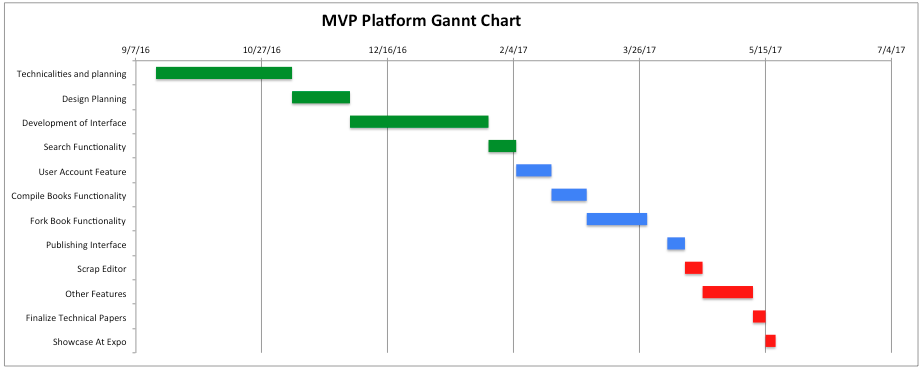
\includegraphics[width=160mm]{gantt_chart.png}
\caption{A simple preliminary Gantt Chart}
\end{figure}

\clearpage\setcounter{page}{1}\pagestyle{Convertviii}
\section[APPENDIX B. \ UML Diagram]{\selectlanguage{english}\rmfamily\bfseries\color{black}
APPENDIX B. \ Unified Modeling Language Diagram}

\bigskip

%\noindent {\selectlanguage{english}\color{black}
%[ insert appendix B here ]}

\begin{figure}[ht!]
\centering
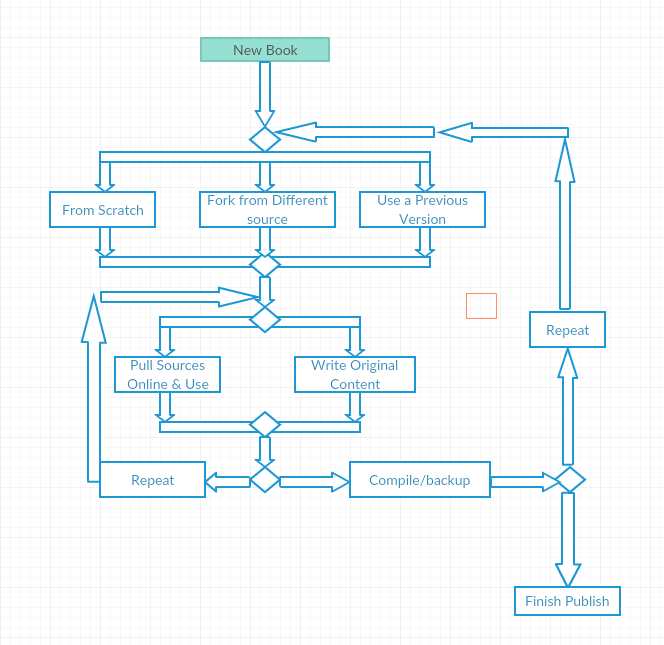
\includegraphics[width=150mm]{usage_diagram.png}
\caption{A preliminary Usage Diagram}
\end{figure}

\bigskip

\newpage
\centerline{\sc \large Signature Page}
\vspace{5pc}


\centering

\begin{tabular}{lllll}
Dr. Carlos Jensen, Client    & \_\_\_\_\_\_\_\_\_\_\_\_\_\_\_\_\_\_\_\_\_\_\_\_\_\_\_\_\_\_\_\_\_\_ & Date & \_\_\_\_\_\_\_\_\_\_\_\_\_\_\_\_\_\_\_\_\_ &  \\
                         &                                                                                  &      &                                            &  \\ \\
Steven Powers, Developer & \_\_\_\_\_\_\_\_\_\_\_\_\_\_\_\_\_\_\_\_\_\_\_\_\_\_\_\_\_\_\_\_\_\_ & Date & \_\_\_\_\_\_\_\_\_\_\_\_\_\_\_\_\_\_\_\_\_ &  \\ 
                         &                                                                                  &      &                                            &  \\ \\
Josh Matteson, Developer & \_\_\_\_\_\_\_\_\_\_\_\_\_\_\_\_\_\_\_\_\_\_\_\_\_\_\_\_\_\_\_\_\_\_ & Date & \_\_\_\_\_\_\_\_\_\_\_\_\_\_\_\_\_\_\_\_\_ &  \\ 
                         &                                                                                  &      &                                            &  \\ \\
Evan Tschuy, Developer   & \_\_\_\_\_\_\_\_\_\_\_\_\_\_\_\_\_\_\_\_\_\_\_\_\_\_\_\_\_\_\_\_\_\_ & Date & \_\_\_\_\_\_\_\_\_\_\_\_\_\_\_\_\_\_\_\_\_ &  \\ 
                         &                                                                                  &      &                                            & 
\end{tabular}

\end{document}
